\documentclass{article}
\usepackage{graphicx} % Required for inserting images
\usepackage{hyperref}

\title{Pendolo quadrifilare}
\author{Francesco Angelo Fabiano Antonacci \\ Alessandro Di Meglio}
\date{\today}

\begin{document}
\maketitle
\section{Scopo dell'esperienza}
Gli scopi dell'esperienza sono:

\begin{itemize}
\item lo studio della costante di smorzamento della velocità di oscillazione del pendolo 
\item studio della dipendenza del periodo dall'ampiezza di oscillazione
\end{itemize}




\section{Cenni teorici}

Ai fini di stimare le velocità massime $v_{max}$ nel punto più basso è stata utilizzata la seguente relazione:

\begin{equation}
v_{max}= \frac{w l}{t_T d}
\label{eq:vmax}
\end{equation}

Dove $w$ è l'ampiezza della bandierina, $l$ è la distanza centro di massa-punto di sospensione, $t_T$ è il tempo che la bandierina impiega per passare attraverso il sensore, $d$ è la distanza tra punto di sospensione-bandierina.




Assunto che l'attrito viscoso sia proporzionale alla velocità massima $v(t)$ con la quale un pendolo oscilla, la $v(t)$  decresce esponenzialmente con un coefficiente di smorzamento $\lambda$. Data $v_0$ la velocità iniziale è valida:  

\begin{equation}
v(t) = v_0 e^{\lambda t}
\label{eq:vt}
\end{equation}

Definiamo il tempo di smorzamento come $\tau=\frac{1}{\lambda}$.

L'ampiezza massima  di ciascuna oscillazione è stata stimata con la seguente relazione:
\begin{equation}
\theta = \arccos(1-\frac{v_{max}^2}{2gl})
\label{eq:thmax}
\end{equation}

Dove  $g $ è l'accelerazione di gravità.
Il periodo delle oscillazioni di un pendolo in funzione dell'ampiezza delle oscillazioni è descritto dalla seguente equazione:

\begin{equation}
T = \sqrt{\frac{d}{g}} (a_1+a_2\theta^2+a_3\theta^4+ o( \theta^4 ))
\label{eq:tht}
\end{equation}
Dove è possibile dimostrare che $a_1=1$, $a_2=\frac{1}{16}$, $a_3=\frac{11}{3072}$.






\section{Apparato strumentale}

\subsection{Materiale}

\begin{itemize}
\item  Un pendolo quadrifilare;
\item  un computer per acquisizione ed analisi dei dati.
\end{itemize}

\subsection{Strumenti di misura}

\begin{itemize}
\item  calibro  ventesimale (risoluzione $ 0.05 mm$ )
\item  metro a nastro (risoluzione $1 mm$)
\item Arduino (risoluzione $1\mu s$)
\end{itemize}





\section{Descrizione delle misure}


In tabella($\ref{tab:dimpar}$) riportiamo le misure raccolte relative alle dimensioni del pendolo.
\begin{table}[h!]
		\centering
		\begin{tabular}{|ccc|}
			\hline
			$b $[mm] & $l$[mm] & $w$[mm]	\\
			$58 \pm 1$	 & 	$	1087\pm1$ 	& $19.80\pm0.05$\\
			\hline
			
		\end{tabular}
		
		\label{tab:dimpar}	
		\caption{$b$ è la distanza tra centro di massa e bandierina, $l$ la distanza tra centro di massa del pendolo e  punto di sospensione, $w$ è lo spessore della bandierina.} 


\end{table}

E' stato lasciato oscillare il pendolo più volte e partendo da diverse ampeizze iniziali e da Arduino sono stati acquisiti: tempo di transito, periodo di oscillazione, tempo rispetto all'avvio delle misure.





\section{Analisi dei dati}

\subsection{Smorzamento della velocità di oscillazione}
\label{sez:vt}

Si fa un fit ai minimi quadrati dell'equazione ($\ref{eq:vt}$) lasciando $v_0$ e $\lambda$ come parametri liberi.
Si verifica che l'influenza dell'incertezza sui tempi è cinque ordini di grandezza più piccola dell'incertezza sulle velocità misurate: di conseguenza i tempi saranno la variabile indipendente.
In tabella ($\ref{tab:vt}$) sono riportati i risultati dell'algoritmo di best-fit.

\begin{table}[h!]
		\centering
		\begin{tabular}{|ccc|}
			\hline

			$v_0$ [m/s] &  $\lambda [s^{-1}$] & $\tau[s]$ 	\\
			$0.4967 \pm 0.0001$	 & 	$2533 10^{-6} \pm 2 10^{-6}$ 	& $394.8\pm0.3$\\
			\hline
			
		\end{tabular}
		
		\label{tab:vt}	
		\caption{Risultati dell'algoritmo di best fit per l'equazione($\ref{eq:vt}$)} 
\end{table}

In figura(\ref{fig:vt}) sono riportati i dati sperimentali considerati in questa sezione e la previsione del modello teorico, in figura (\ref{fig:vtres}) è riportato il grafico dei residui.

\begin{figure}[h!]
	\includegraphics[width=\textwidth]{plot_exp.png}
	\caption{Dati sperimentali e previsione del modello teorico coi parametri di best-fit.}
	\label{fig:vt}
\end{figure}

\begin{figure}[h!]
	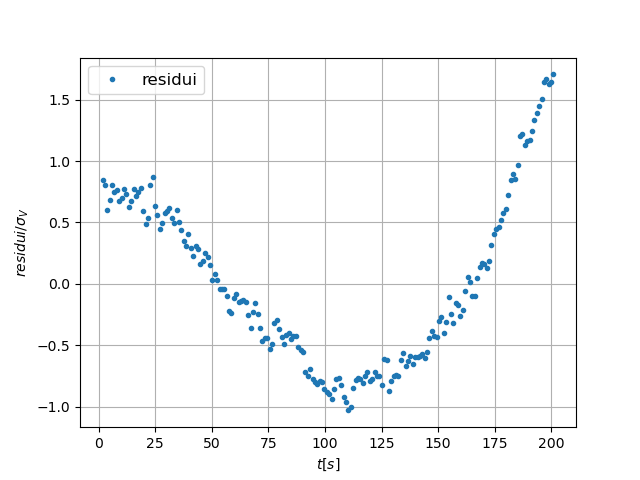
\includegraphics[width=\textwidth]{Residuals_exponential_law.png}
	\caption{Grafico dei residui della legge(\ref{eq:vt}).}
	\label{fig:vtres}
\end{figure}


\subsubsection{Valutazione del modello}

Dal grafico dei residui, a causa delle eccessive permanenze,  si deduce la presenza di un errore sistematico o di un errore del modello.
Segue che non è possibile fare il test del $\chi^2$. 

\subsection{Variazione del periodo in funzione dell'angolo massimo}

E' stato ripetuto il fit descritto nella sezione($\ref{sez:vt}$) su un campionameto di dati diverso, per poter considerare oscillazioni di maggiore ampiezza. Grazie alla relazione($\ref{eq:thmax}$) è stata fatta la stima degli angoli massimi.
E' stato fatto il fit ai minimi quadrati dell'equazione ($\ref{eq:tht}$) lasciando come parametri liberi $k=\frac{l}{g}$, ma anche $a_1$,$a_2$,$a_3$.
Come variabile indipendente è stato utilizzato l'angolo massimo, stimato secondo l'equazione($\ref{eq:thmax}$); come variabile dipendende sono stati utilizzati i periodi registrati da Arduino.
Non essendo trascurabili gli errori sulla variabile indipendente è stato utilizzato l'errore efficace iterando l'algoritmo di best-fit.

In tabella ($\ref{tab:tht}$) sono riportati i risultati dell'algoritmo di best-fit.

\begin{table}[h!]


	\centering
		\begin{tabular}{|cc|}
		\hline

			$v_0 [m/s]$ & $ 2.6605\pm0.0008$ \\
			$\lambda[s^{-1}]$ & $-0.003305\pm 0.000005$\\
			$k[s]$ & $0.12\pm60$\\
			$a_1$ &  $0.96\pm240$\\
			$a_2$ & $0.061\pm15$\\
			$a_3$ & $0.00423\pm1$\\

		\hline


		\end{tabular}
	\caption{Risultati dell'algoritmo di best fit per l'equazione($\ref{eq:tht}$)}
	\label{tab:tht}

\end{table}

E' stato osservato che se utilizzare tre termini anziché due nello sviluppo della formula del periodo delle oscillazioni del pendolo (equazione($\ref{eq:tht}$)) migliora sensibilmente i residui, aggiungerne un quarto non fa altrettanto:inoltre già il terzo termine dello sviluppo si inizia a discostare dal valore previsto dalla teoria.

\begin{figure}[h!]
	\includegraphics[width=\textwidth]{plot_Periods-time.png}
	\caption{Periodo di oscillazione del pendolo in funzione del tempo trascorso.}
	\label{fig:pt}
\end{figure}

\begin{figure}[h!]
	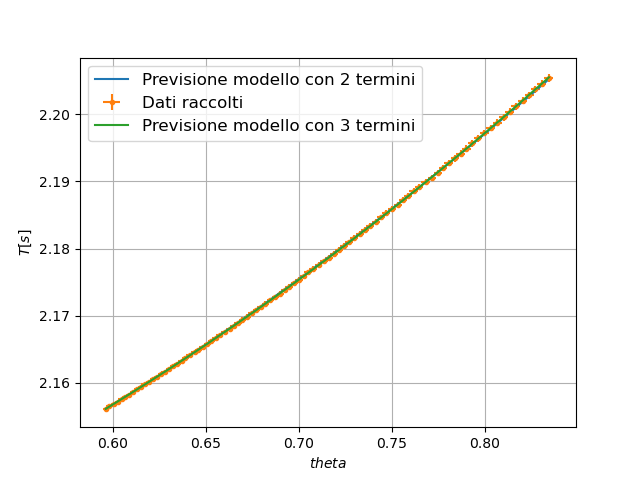
\includegraphics[width=\textwidth]{Plot_Periods-Theta.png}
	\caption{Periodo del pendolo in funzione dell'apertura massima}
	\label{fig:pth}
\end{figure}

\begin{figure}[h!]
	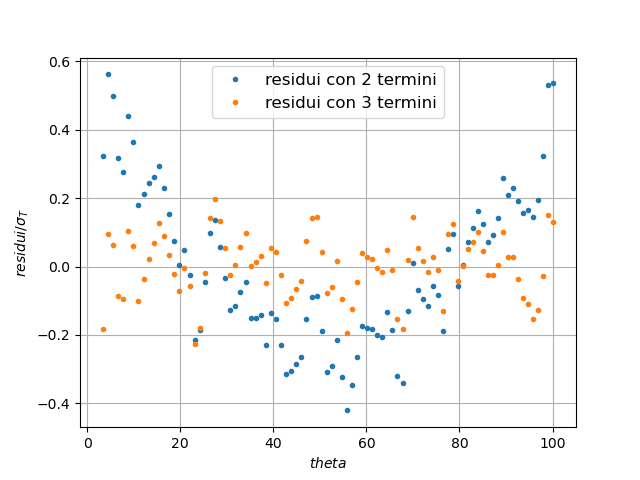
\includegraphics[width=\textwidth]{Residuals_period_law.png}
	\caption{Grafico dei residui della legge(\ref{eq:tht}).}
	\label{fig:ptres}
\end{figure}


\subsubsection{Valutazione del modello}

Dal grafico dei residui non vi è motivo di rigettare il modello.
Ciononostante  $\chi^2=28$ , $p_{value}=10^{-8}$, $Dof=88$; segue o che gli errori sono stati sovrastimati, oppure che il modello di fit è stato troppo flessibile.


\section{Conclusione}









\end{document}
